\documentclass[a4paper,11pt]{article}
\usepackage[T1]{fontenc}

%opening
\title{\texttt{fcc\_analyzer\_PyQt5}\\ a GUI to visualize \fcc\ output}
\date{\textsc{Version: 0.1}\\\today}
\author{Javier Cerezo\\\href{mailto:javier.cerezo@uam.es}{\texttt{javier.cerezo@uam.es}}}

% Margins
\textheight 22.0cm \textwidth 14.7cm \oddsidemargin 1cm
\evensidemargin 1cm \topmargin -0.25cm

%Packages
\usepackage{graphics}
\usepackage[pdftex]{graphicx}

\usepackage{amsmath}
\usepackage{amssymb}
\usepackage{color}
\usepackage{xcolor}

\usepackage{hyperref}
% The following metadata will show up in the PDF properties
\hypersetup{
  colorlinks = true,
  urlcolor = blue,
}


\begin{document}
\setlength{\parskip}{0.5em}
\newcommand{\fcc}{$\mathcal{FC}$\textit{classes}}

\maketitle

\section{Description}
\texttt{fcc\_analyzer\_PyQt5} is a graphical user interface (GUI) written in python3 and relying on the PyQt5 and matplotlib libraries. It reads the output from \fcc\ (for a TI calculation), namely fort.21/Assigments.dat (assignments) and either fort.22/Bin\_Spectrum.dat (spectral histogram) or fort.18 (final convoluted spectrum), and opens an interactive plot that facilitates the analysis of the transitions, the investigation of different broadening schemes (if fort.22/Bin\_Spectrum.dat is available) and the comparison with reference spectral data.

\section{Installation}

\subsection{Precompiled binary}
System-specific binaries generated with \texttt{cx-Freeze} or \texttt{pyinstaller} may be available from the author upon request.

\subsection{Python script}
The source can be run directly as a python script from any computer architechture where a python interpreter is available. The python script is located in \texttt{src/}. \texttt{python} version 3 is required along with following modules (the minimum version tested is specified):

\begin{itemize}
 \item \texttt{matplotlib} (version $\geq1.4.2$)
 \item \texttt{numpy} (version $\geq1.9.1$)
\end{itemize}

PyQt binding are also needed, as provided through the module PyQt5\footnote{A version relying on PyQt4 is also available but is deprecated and no loger mantained. It requires python 2.7.}

\begin{itemize}
 \item \texttt{PyQt5} (version $\geq5.9.2$)
\end{itemize}

% \clearpage

One of the most straightfoward methods to get a working python environment is through the \href{http://conda.pydata.org/docs/intro.html}{\texttt{conda}} package manager, which allows to install and manage different python versions easily. Among the advantages, it can be installed at the user folders/account not requiring admin (or root) privileges and it is available for different operating systems as a simple installer. A very suitable package for conda is miniconda, a light-weight version that can be downloaded from \href{https://docs.conda.io/en/latest/miniconda.html}{\texttt{https://docs.conda.io/en/latest/miniconda.html}}.

Once installed, the required modules to run the \texttt{fcc\_analyzer\_PyQt5} script can be installed through the command line (under any of the supported operating systems) by simply typing:\\

\texttt{conda install pyqt numpy matplotlib python=3}\\

The user is refered to the oficial \texttt{conda} documentation for further details.

% \clearpage

\section{Running the application}

\subsection{Launch the application}
The application should be invoked in the folder were the fort.21 and either fort.22 or fort.18 files that will be analysed reside, using the following syntax from the command line:\\

\texttt{fcc\_analyzer\_PyQt5 [flags]}\\

If no fort.21 is found in the current directory, a dialog to set the path to the files will be opened (this is useful when the program is called by mouser-clicking, e.g. in Windows). The following optional flags can be used when called from the command line:

\begin{tabular}{lll}
 \texttt{-type (abs|emi|ecd|cpl)}     && \begin{minipage}[t]{0.65\textwidth}
                                          Type of {\fcc} calculation performed.
                                         \end{minipage}\\\\
 \texttt{-maxC N}                     && \begin{minipage}[t]{0.65\textwidth}
                                          Maximum class to by loaded (\texttt{N}$\leq7$).
                                         \end{minipage}\\\\
 \texttt{-h}                          && \begin{minipage}[t]{0.65\textwidth}
                                          Show help.
                                         \end{minipage}\\\\
\end{tabular}

\clearpage

\subsection{Using the application}
The GUI consists of the following parts:

\begin{figure}[h!]
\begin{center}
  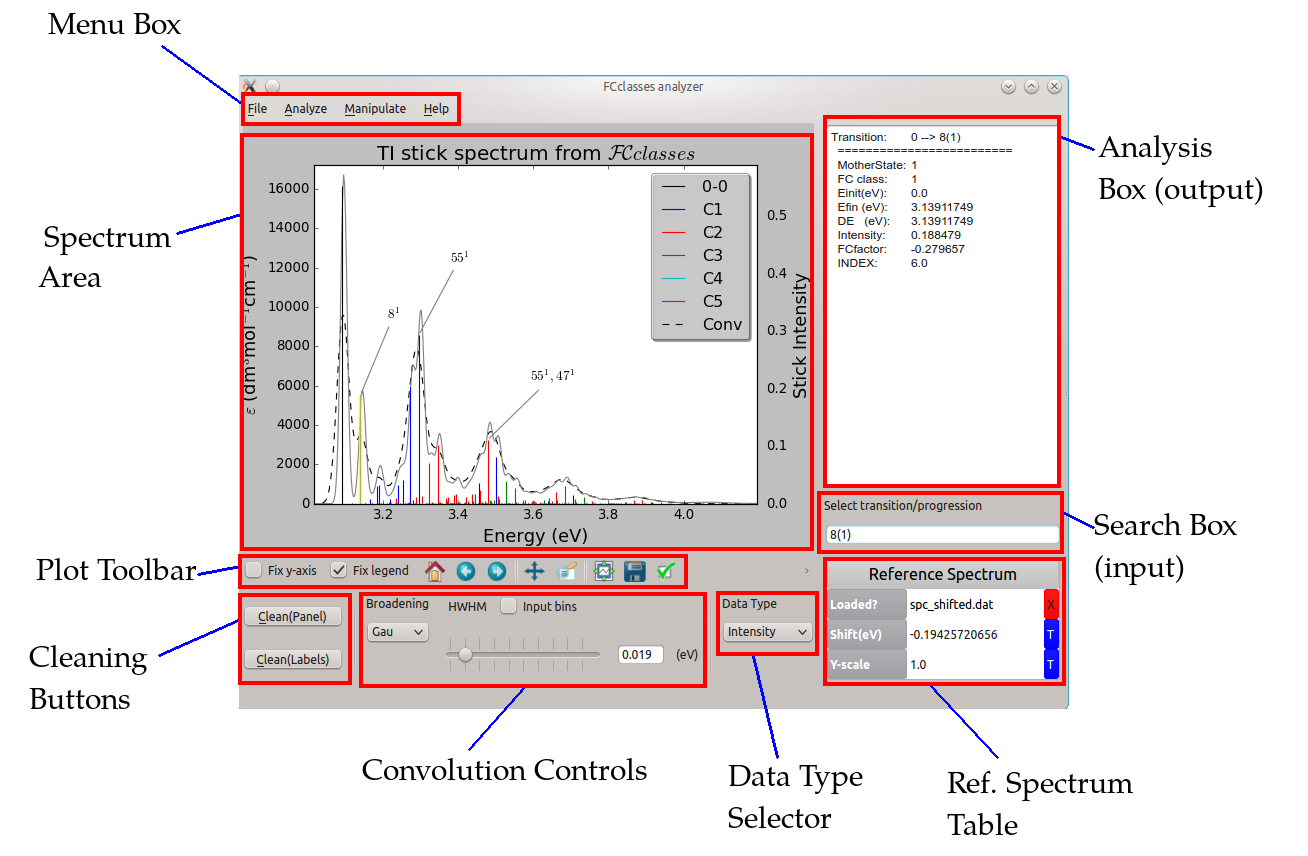
\includegraphics[width=15cm]{figs/fcc_analyzer_screeshot.png}
\end{center}
\caption{Screenshot of \texttt{fcc\_analyzer\_PyQt5} highlighting the different parts.}
\end{figure}

The interaction and analysis of the simulated spectrum are performed with the different widgets in the plot. Below, the different parts are described.

\subsubsection{Menu Box}
\begin{itemize}
 \item File
 \begin{itemize}
  \item Save plot: save plot to a png file.
  \item Export to xmgrace: export plot data (including labels) to xmgrace file. A export assistant is first raised to select how to organize the plots:
  \begin{itemize}
   \item Overlaid graphs: place the stick and spectra in different graphs, that are overlaid, as in the matplotlib plot.
   \item Same graph: include sticks and spectra in the same graph. The spectra are normalized to the maximum stick intensity.
  \end{itemize}

  \item Import plot: Load reference spectrum to the Spectrum Area. Units: (eV|cm$^{-1}$|nm).
  \item Quit: exit the application
 \end{itemize}

 \item Analyse
 \begin{itemize}
  \item Momenta: compute momenta of the convoluted and write to the Analysis Box.
 \end{itemize}

 \item Manipulate
 \begin{itemize}
  \item Shift to simulated: shift reference spectrum (if loaded) to match the convoluted spectrum.
  \item Scale to convoluted: scale reference spectrum (if loaded) to match the convoluted spectrum.
 \end{itemize}

 \item Help
 \begin{itemize}
  \item Instructions: show a short guide to use the application.
  \item About: show general info about the application.
 \end{itemize}
\end{itemize}
 
\subsubsection{Spectrum Area}
This area is interactive. The following actions are possible:
\begin{itemize}
 \item Right-mouse click on a stick: highlight and get info about the transition (written into Analysis Box).
 \item Left-mouse click on a stick: add label over the stick
 \item Right-mouse click on a label: drag the label
 \item Right-mouse click on a legend line: activate/deactivate plot
 \item Press ``+''/``-'' keys to browse back and forward between highlighted stick
\end{itemize}

\subsubsection{Analysis Box}
In this box, the information about the highlighted transitions is shown, as well as the analysis of the momenta. This box is not editable, but the info can be copied.

\subsubsection{Search Box}
Selector of transitions. The general syntax is the following:

{
\scriptsize
\texttt{Mode1'(Quanta1'),Mode2'(Quanta2')... {-}{-}> Mode1(Quanta1),Mode2(Quanta2)...}
}\\

where \texttt{Mode1'(Quanta1')} refer to mode \texttt{Mode1'} in the initial state that is excited \texttt{Quanta1'} quanta, and \texttt{Mode1(Quanta1)} are the equivalent entities for the final state.

The ground vibrational state is represented by a zero (\texttt{0}). When the initial state is in the ground state, the initial part, \texttt{0{-}{-}>} can be omitted. Some examples:

\begin{itemize}
 \item \texttt{8(1),9(2)}: select the transition from the ground initial state to the final state where mode 8 is excited 1 quantum and mode 9 is excited 2 quanta.
 \item \texttt{0{-}{-}>8(1),9(2)}: same as above
 \item \texttt{8(1){-}{-}>0}: select transition from initial state excited 1 quantum on mode 8 to the final ground state.
 \item \texttt{0{-}{-}>0}: select 0-0 transition
\end{itemize}

To select a progression in the final state, use \texttt{P} instead of the number of quanta. This keyword can only be used for one mode in the same selection. Some examples:

\begin{itemize}
 \item \texttt{8(p)}: select progression of mode 8 in the final state.
 \item \texttt{0{-}{-}>8(p),9(2)}: select progression of mode 8 in the final state when, simultaneously, mode 9 is excited 2 quanta.
 \item \texttt{1(1){-}{-}>8(p)}: select progression of mode 8 in the final state, starting from the initial state where mode 1 is excited one quantum.
\end{itemize}

\subsubsection{Plot Toolbar}
This is formed by two check boxes and the standard matplotlib toolbar with PyQt5 back-end. The check boxes are:
\begin{itemize}
 \item Fix y-axis: whether or not scale y-axis when the convolution or the data type are updated.
 \item Fix legend: whether the legend can be displaced with the mouse of not.
\end{itemize}

The matplotlib toolbar include:
\begin{itemize}
 \item 
\includegraphics[width=0.5cm]{figs/butt_zoom.jpg}: zoom into (left mouse click) or out (right mouse click) a rectangle.
 \item 
\includegraphics[width=0.5cm]{figs/butt_move.jpg}: move the spectrum (left mouse click) or zoom (right mouse click).
 \item 
\includegraphics[width=0.5cm]{figs/butt_save.jpg}: export image.
 \item 
\includegraphics[width=0.5cm]{figs/butt_edit.jpg}: customize axes properties.
\end{itemize}

\subsubsection{Cleaning Buttons}
\begin{itemize}
 \item Clean(Panel): remove highlight on transitions and clear the analysis box.
 \item Clean(Labels): clear all labels added to the spectrum
\end{itemize}

\subsubsection{Convolution Controls}
These controls are only active if the fort.22 file is available. Note that this is not present for old versions of \fcc.
\begin{itemize}
 \item Broadening selector [Gau|Lor]: type of broadening function
 \item HWHM slider and box: set the HWHM of the broadening function. The box is editable and allows a more precise selection of the value, even beyond the slider limits (0.01 to 0.1\,eV).
 \item Input bins check box: use the bins given in the input fort.22 file. Otherwise, a new histogram with only 1000 bins is used (which is faster).
\end{itemize}

\subsubsection{Data Type Selector}
Select the type of spectrum: [Intensity|Lineshape].

\subsubsection{Ref. Spectrum Table}
Information about the reference spectrum (loaded with File->Import plot).

\begin{itemize}
 \item Loaded?: whether reference spectrum is loaded. If so the file name is shown. The red button with the cross deletes the reference spectrum.
 \item Shift(eV): shift applied to the reference spectrum (in eV). This box is editable. The value always refer to the originally loaded value, unless the blue T button is pressed, which resets the reference value to the current one.
 \item Y-scale: scaling applied to the reference spectrum Y-axis. This box is editable. The value always refer to the originally loaded value, unless the blue T button is pressed, which resets the reference value to the current one.
\end{itemize}


\end{document}
